\documentclass[11pt]{article}

    \usepackage{tabularx}
    \usepackage[breakable]{tcolorbox}
    \usepackage{parskip} % Stop auto-indenting (to mimic markdown behaviour)
    
    \usepackage{iftex}
    \ifPDFTeX
    	\usepackage[T1]{fontenc}
    	\usepackage{mathpazo}
    \else
    	\usepackage{fontspec}
    \fi

    % Basic figure setup, for now with no caption control since it's done
    % automatically by Pandoc (which extracts ![](path) syntax from Markdown).
    \usepackage{graphicx}
    % Maintain compatibility with old templates. Remove in nbconvert 6.0
    \let\Oldincludegraphics\includegraphics
    % Ensure that by default, figures have no caption (until we provide a
    % proper Figure object with a Caption API and a way to capture that
    % in the conversion process - todo).
    \usepackage{caption}
    \DeclareCaptionFormat{nocaption}{}
    \captionsetup{format=nocaption,aboveskip=0pt,belowskip=0pt}

    \usepackage[Export]{adjustbox} % Used to constrain images to a maximum size
    \adjustboxset{max size={0.9\linewidth}{0.9\paperheight}}
    \usepackage{float}
    \floatplacement{figure}{H} % forces figures to be placed at the correct location
    \usepackage{xcolor} % Allow colors to be defined
    \usepackage{enumerate} % Needed for markdown enumerations to work
    \usepackage{geometry} % Used to adjust the document margins
    \usepackage{amsmath} % Equations
    \usepackage{amssymb} % Equations
    \usepackage{textcomp} % defines textquotesingle
    % Hack from http://tex.stackexchange.com/a/47451/13684:
    \AtBeginDocument{%
        \def\PYZsq{\textquotesingle}% Upright quotes in Pygmentized code
    }
    \usepackage{upquote} % Upright quotes for verbatim code
    \usepackage{eurosym} % defines \euro
    \usepackage[mathletters]{ucs} % Extended unicode (utf-8) support
    \usepackage{fancyvrb} % verbatim replacement that allows latex

    % The hyperref package gives us a pdf with properly built
    % internal navigation ('pdf bookmarks' for the table of contents,
    % internal cross-reference links, web links for URLs, etc.)
    \usepackage{hyperref}
    % The default LaTeX title has an obnoxious amount of whitespace. By default,
    % titling removes some of it. It also provides customization options.
    \usepackage{titling}
    \usepackage{longtable} % longtable support required by pandoc >1.10
    \usepackage{booktabs}  % table support for pandoc > 1.12.2
    \usepackage[inline]{enumitem} % IRkernel/repr support (it uses the enumerate* environment)
    \usepackage[normalem]{ulem} % ulem is needed to support strikethroughs (\sout)
                                % normalem makes italics be italics, not underlines
    \usepackage{mathrsfs}
    

    
    % Colors for the hyperref package
    \definecolor{urlcolor}{rgb}{0,.145,.698}
    \definecolor{linkcolor}{rgb}{.71,0.21,0.01}
    \definecolor{citecolor}{rgb}{.12,.54,.11}

    % ANSI colors
    \definecolor{ansi-black}{HTML}{3E424D}
    \definecolor{ansi-black-intense}{HTML}{282C36}
    \definecolor{ansi-red}{HTML}{E75C58}
    \definecolor{ansi-red-intense}{HTML}{B22B31}
    \definecolor{ansi-green}{HTML}{00A250}
    \definecolor{ansi-green-intense}{HTML}{007427}
    \definecolor{ansi-yellow}{HTML}{DDB62B}
    \definecolor{ansi-yellow-intense}{HTML}{B27D12}
    \definecolor{ansi-blue}{HTML}{208FFB}
    \definecolor{ansi-blue-intense}{HTML}{0065CA}
    \definecolor{ansi-magenta}{HTML}{D160C4}
    \definecolor{ansi-magenta-intense}{HTML}{A03196}
    \definecolor{ansi-cyan}{HTML}{60C6C8}
    \definecolor{ansi-cyan-intense}{HTML}{258F8F}
    \definecolor{ansi-white}{HTML}{C5C1B4}
    \definecolor{ansi-white-intense}{HTML}{A1A6B2}
    \definecolor{ansi-default-inverse-fg}{HTML}{FFFFFF}
    \definecolor{ansi-default-inverse-bg}{HTML}{000000}

    % commands and environments needed by pandoc snippets
    % extracted from the output of `pandoc -s`
    \providecommand{\tightlist}{%
      \setlength{\itemsep}{0pt}\setlength{\parskip}{0pt}}
    \DefineVerbatimEnvironment{Highlighting}{Verbatim}{commandchars=\\\{\}}
    % Add ',fontsize=\small' for more characters per line
    \newenvironment{Shaded}{}{}
    \newcommand{\KeywordTok}[1]{\textcolor[rgb]{0.00,0.44,0.13}{\textbf{{#1}}}}
    \newcommand{\DataTypeTok}[1]{\textcolor[rgb]{0.56,0.13,0.00}{{#1}}}
    \newcommand{\DecValTok}[1]{\textcolor[rgb]{0.25,0.63,0.44}{{#1}}}
    \newcommand{\BaseNTok}[1]{\textcolor[rgb]{0.25,0.63,0.44}{{#1}}}
    \newcommand{\FloatTok}[1]{\textcolor[rgb]{0.25,0.63,0.44}{{#1}}}
    \newcommand{\CharTok}[1]{\textcolor[rgb]{0.25,0.44,0.63}{{#1}}}
    \newcommand{\StringTok}[1]{\textcolor[rgb]{0.25,0.44,0.63}{{#1}}}
    \newcommand{\CommentTok}[1]{\textcolor[rgb]{0.38,0.63,0.69}{\textit{{#1}}}}
    \newcommand{\OtherTok}[1]{\textcolor[rgb]{0.00,0.44,0.13}{{#1}}}
    \newcommand{\AlertTok}[1]{\textcolor[rgb]{1.00,0.00,0.00}{\textbf{{#1}}}}
    \newcommand{\FunctionTok}[1]{\textcolor[rgb]{0.02,0.16,0.49}{{#1}}}
    \newcommand{\RegionMarkerTok}[1]{{#1}}
    \newcommand{\ErrorTok}[1]{\textcolor[rgb]{1.00,0.00,0.00}{\textbf{{#1}}}}
    \newcommand{\NormalTok}[1]{{#1}}
    
    % Additional commands for more recent versions of Pandoc
    \newcommand{\ConstantTok}[1]{\textcolor[rgb]{0.53,0.00,0.00}{{#1}}}
    \newcommand{\SpecialCharTok}[1]{\textcolor[rgb]{0.25,0.44,0.63}{{#1}}}
    \newcommand{\VerbatimStringTok}[1]{\textcolor[rgb]{0.25,0.44,0.63}{{#1}}}
    \newcommand{\SpecialStringTok}[1]{\textcolor[rgb]{0.73,0.40,0.53}{{#1}}}
    \newcommand{\ImportTok}[1]{{#1}}
    \newcommand{\DocumentationTok}[1]{\textcolor[rgb]{0.73,0.13,0.13}{\textit{{#1}}}}
    \newcommand{\AnnotationTok}[1]{\textcolor[rgb]{0.38,0.63,0.69}{\textbf{\textit{{#1}}}}}
    \newcommand{\CommentVarTok}[1]{\textcolor[rgb]{0.38,0.63,0.69}{\textbf{\textit{{#1}}}}}
    \newcommand{\VariableTok}[1]{\textcolor[rgb]{0.10,0.09,0.49}{{#1}}}
    \newcommand{\ControlFlowTok}[1]{\textcolor[rgb]{0.00,0.44,0.13}{\textbf{{#1}}}}
    \newcommand{\OperatorTok}[1]{\textcolor[rgb]{0.40,0.40,0.40}{{#1}}}
    \newcommand{\BuiltInTok}[1]{{#1}}
    \newcommand{\ExtensionTok}[1]{{#1}}
    \newcommand{\PreprocessorTok}[1]{\textcolor[rgb]{0.74,0.48,0.00}{{#1}}}
    \newcommand{\AttributeTok}[1]{\textcolor[rgb]{0.49,0.56,0.16}{{#1}}}
    \newcommand{\InformationTok}[1]{\textcolor[rgb]{0.38,0.63,0.69}{\textbf{\textit{{#1}}}}}
    \newcommand{\WarningTok}[1]{\textcolor[rgb]{0.38,0.63,0.69}{\textbf{\textit{{#1}}}}}
    
    
    % Define a nice break command that doesn't care if a line doesn't already
    % exist.
    \def\br{\hspace*{\fill} \\* }
    % Math Jax compatibility definitions
    \def\gt{>}
    \def\lt{<}
    \let\Oldtex\TeX
    \let\Oldlatex\LaTeX
    \renewcommand{\TeX}{\textrm{\Oldtex}}
    \renewcommand{\LaTeX}{\textrm{\Oldlatex}}
    % Document parameters
    % Document title
    \title{U5A1-K-means\_clustering}
    
    
    
    
    
% Pygments definitions
\makeatletter
\def\PY@reset{\let\PY@it=\relax \let\PY@bf=\relax%
    \let\PY@ul=\relax \let\PY@tc=\relax%
    \let\PY@bc=\relax \let\PY@ff=\relax}
\def\PY@tok#1{\csname PY@tok@#1\endcsname}
\def\PY@toks#1+{\ifx\relax#1\empty\else%
    \PY@tok{#1}\expandafter\PY@toks\fi}
\def\PY@do#1{\PY@bc{\PY@tc{\PY@ul{%
    \PY@it{\PY@bf{\PY@ff{#1}}}}}}}
\def\PY#1#2{\PY@reset\PY@toks#1+\relax+\PY@do{#2}}

\expandafter\def\csname PY@tok@w\endcsname{\def\PY@tc##1{\textcolor[rgb]{0.73,0.73,0.73}{##1}}}
\expandafter\def\csname PY@tok@c\endcsname{\let\PY@it=\textit\def\PY@tc##1{\textcolor[rgb]{0.25,0.50,0.50}{##1}}}
\expandafter\def\csname PY@tok@cp\endcsname{\def\PY@tc##1{\textcolor[rgb]{0.74,0.48,0.00}{##1}}}
\expandafter\def\csname PY@tok@k\endcsname{\let\PY@bf=\textbf\def\PY@tc##1{\textcolor[rgb]{0.00,0.50,0.00}{##1}}}
\expandafter\def\csname PY@tok@kp\endcsname{\def\PY@tc##1{\textcolor[rgb]{0.00,0.50,0.00}{##1}}}
\expandafter\def\csname PY@tok@kt\endcsname{\def\PY@tc##1{\textcolor[rgb]{0.69,0.00,0.25}{##1}}}
\expandafter\def\csname PY@tok@o\endcsname{\def\PY@tc##1{\textcolor[rgb]{0.40,0.40,0.40}{##1}}}
\expandafter\def\csname PY@tok@ow\endcsname{\let\PY@bf=\textbf\def\PY@tc##1{\textcolor[rgb]{0.67,0.13,1.00}{##1}}}
\expandafter\def\csname PY@tok@nb\endcsname{\def\PY@tc##1{\textcolor[rgb]{0.00,0.50,0.00}{##1}}}
\expandafter\def\csname PY@tok@nf\endcsname{\def\PY@tc##1{\textcolor[rgb]{0.00,0.00,1.00}{##1}}}
\expandafter\def\csname PY@tok@nc\endcsname{\let\PY@bf=\textbf\def\PY@tc##1{\textcolor[rgb]{0.00,0.00,1.00}{##1}}}
\expandafter\def\csname PY@tok@nn\endcsname{\let\PY@bf=\textbf\def\PY@tc##1{\textcolor[rgb]{0.00,0.00,1.00}{##1}}}
\expandafter\def\csname PY@tok@ne\endcsname{\let\PY@bf=\textbf\def\PY@tc##1{\textcolor[rgb]{0.82,0.25,0.23}{##1}}}
\expandafter\def\csname PY@tok@nv\endcsname{\def\PY@tc##1{\textcolor[rgb]{0.10,0.09,0.49}{##1}}}
\expandafter\def\csname PY@tok@no\endcsname{\def\PY@tc##1{\textcolor[rgb]{0.53,0.00,0.00}{##1}}}
\expandafter\def\csname PY@tok@nl\endcsname{\def\PY@tc##1{\textcolor[rgb]{0.63,0.63,0.00}{##1}}}
\expandafter\def\csname PY@tok@ni\endcsname{\let\PY@bf=\textbf\def\PY@tc##1{\textcolor[rgb]{0.60,0.60,0.60}{##1}}}
\expandafter\def\csname PY@tok@na\endcsname{\def\PY@tc##1{\textcolor[rgb]{0.49,0.56,0.16}{##1}}}
\expandafter\def\csname PY@tok@nt\endcsname{\let\PY@bf=\textbf\def\PY@tc##1{\textcolor[rgb]{0.00,0.50,0.00}{##1}}}
\expandafter\def\csname PY@tok@nd\endcsname{\def\PY@tc##1{\textcolor[rgb]{0.67,0.13,1.00}{##1}}}
\expandafter\def\csname PY@tok@s\endcsname{\def\PY@tc##1{\textcolor[rgb]{0.73,0.13,0.13}{##1}}}
\expandafter\def\csname PY@tok@sd\endcsname{\let\PY@it=\textit\def\PY@tc##1{\textcolor[rgb]{0.73,0.13,0.13}{##1}}}
\expandafter\def\csname PY@tok@si\endcsname{\let\PY@bf=\textbf\def\PY@tc##1{\textcolor[rgb]{0.73,0.40,0.53}{##1}}}
\expandafter\def\csname PY@tok@se\endcsname{\let\PY@bf=\textbf\def\PY@tc##1{\textcolor[rgb]{0.73,0.40,0.13}{##1}}}
\expandafter\def\csname PY@tok@sr\endcsname{\def\PY@tc##1{\textcolor[rgb]{0.73,0.40,0.53}{##1}}}
\expandafter\def\csname PY@tok@ss\endcsname{\def\PY@tc##1{\textcolor[rgb]{0.10,0.09,0.49}{##1}}}
\expandafter\def\csname PY@tok@sx\endcsname{\def\PY@tc##1{\textcolor[rgb]{0.00,0.50,0.00}{##1}}}
\expandafter\def\csname PY@tok@m\endcsname{\def\PY@tc##1{\textcolor[rgb]{0.40,0.40,0.40}{##1}}}
\expandafter\def\csname PY@tok@gh\endcsname{\let\PY@bf=\textbf\def\PY@tc##1{\textcolor[rgb]{0.00,0.00,0.50}{##1}}}
\expandafter\def\csname PY@tok@gu\endcsname{\let\PY@bf=\textbf\def\PY@tc##1{\textcolor[rgb]{0.50,0.00,0.50}{##1}}}
\expandafter\def\csname PY@tok@gd\endcsname{\def\PY@tc##1{\textcolor[rgb]{0.63,0.00,0.00}{##1}}}
\expandafter\def\csname PY@tok@gi\endcsname{\def\PY@tc##1{\textcolor[rgb]{0.00,0.63,0.00}{##1}}}
\expandafter\def\csname PY@tok@gr\endcsname{\def\PY@tc##1{\textcolor[rgb]{1.00,0.00,0.00}{##1}}}
\expandafter\def\csname PY@tok@ge\endcsname{\let\PY@it=\textit}
\expandafter\def\csname PY@tok@gs\endcsname{\let\PY@bf=\textbf}
\expandafter\def\csname PY@tok@gp\endcsname{\let\PY@bf=\textbf\def\PY@tc##1{\textcolor[rgb]{0.00,0.00,0.50}{##1}}}
\expandafter\def\csname PY@tok@go\endcsname{\def\PY@tc##1{\textcolor[rgb]{0.53,0.53,0.53}{##1}}}
\expandafter\def\csname PY@tok@gt\endcsname{\def\PY@tc##1{\textcolor[rgb]{0.00,0.27,0.87}{##1}}}
\expandafter\def\csname PY@tok@err\endcsname{\def\PY@bc##1{\setlength{\fboxsep}{0pt}\fcolorbox[rgb]{1.00,0.00,0.00}{1,1,1}{\strut ##1}}}
\expandafter\def\csname PY@tok@kc\endcsname{\let\PY@bf=\textbf\def\PY@tc##1{\textcolor[rgb]{0.00,0.50,0.00}{##1}}}
\expandafter\def\csname PY@tok@kd\endcsname{\let\PY@bf=\textbf\def\PY@tc##1{\textcolor[rgb]{0.00,0.50,0.00}{##1}}}
\expandafter\def\csname PY@tok@kn\endcsname{\let\PY@bf=\textbf\def\PY@tc##1{\textcolor[rgb]{0.00,0.50,0.00}{##1}}}
\expandafter\def\csname PY@tok@kr\endcsname{\let\PY@bf=\textbf\def\PY@tc##1{\textcolor[rgb]{0.00,0.50,0.00}{##1}}}
\expandafter\def\csname PY@tok@bp\endcsname{\def\PY@tc##1{\textcolor[rgb]{0.00,0.50,0.00}{##1}}}
\expandafter\def\csname PY@tok@fm\endcsname{\def\PY@tc##1{\textcolor[rgb]{0.00,0.00,1.00}{##1}}}
\expandafter\def\csname PY@tok@vc\endcsname{\def\PY@tc##1{\textcolor[rgb]{0.10,0.09,0.49}{##1}}}
\expandafter\def\csname PY@tok@vg\endcsname{\def\PY@tc##1{\textcolor[rgb]{0.10,0.09,0.49}{##1}}}
\expandafter\def\csname PY@tok@vi\endcsname{\def\PY@tc##1{\textcolor[rgb]{0.10,0.09,0.49}{##1}}}
\expandafter\def\csname PY@tok@vm\endcsname{\def\PY@tc##1{\textcolor[rgb]{0.10,0.09,0.49}{##1}}}
\expandafter\def\csname PY@tok@sa\endcsname{\def\PY@tc##1{\textcolor[rgb]{0.73,0.13,0.13}{##1}}}
\expandafter\def\csname PY@tok@sb\endcsname{\def\PY@tc##1{\textcolor[rgb]{0.73,0.13,0.13}{##1}}}
\expandafter\def\csname PY@tok@sc\endcsname{\def\PY@tc##1{\textcolor[rgb]{0.73,0.13,0.13}{##1}}}
\expandafter\def\csname PY@tok@dl\endcsname{\def\PY@tc##1{\textcolor[rgb]{0.73,0.13,0.13}{##1}}}
\expandafter\def\csname PY@tok@s2\endcsname{\def\PY@tc##1{\textcolor[rgb]{0.73,0.13,0.13}{##1}}}
\expandafter\def\csname PY@tok@sh\endcsname{\def\PY@tc##1{\textcolor[rgb]{0.73,0.13,0.13}{##1}}}
\expandafter\def\csname PY@tok@s1\endcsname{\def\PY@tc##1{\textcolor[rgb]{0.73,0.13,0.13}{##1}}}
\expandafter\def\csname PY@tok@mb\endcsname{\def\PY@tc##1{\textcolor[rgb]{0.40,0.40,0.40}{##1}}}
\expandafter\def\csname PY@tok@mf\endcsname{\def\PY@tc##1{\textcolor[rgb]{0.40,0.40,0.40}{##1}}}
\expandafter\def\csname PY@tok@mh\endcsname{\def\PY@tc##1{\textcolor[rgb]{0.40,0.40,0.40}{##1}}}
\expandafter\def\csname PY@tok@mi\endcsname{\def\PY@tc##1{\textcolor[rgb]{0.40,0.40,0.40}{##1}}}
\expandafter\def\csname PY@tok@il\endcsname{\def\PY@tc##1{\textcolor[rgb]{0.40,0.40,0.40}{##1}}}
\expandafter\def\csname PY@tok@mo\endcsname{\def\PY@tc##1{\textcolor[rgb]{0.40,0.40,0.40}{##1}}}
\expandafter\def\csname PY@tok@ch\endcsname{\let\PY@it=\textit\def\PY@tc##1{\textcolor[rgb]{0.25,0.50,0.50}{##1}}}
\expandafter\def\csname PY@tok@cm\endcsname{\let\PY@it=\textit\def\PY@tc##1{\textcolor[rgb]{0.25,0.50,0.50}{##1}}}
\expandafter\def\csname PY@tok@cpf\endcsname{\let\PY@it=\textit\def\PY@tc##1{\textcolor[rgb]{0.25,0.50,0.50}{##1}}}
\expandafter\def\csname PY@tok@c1\endcsname{\let\PY@it=\textit\def\PY@tc##1{\textcolor[rgb]{0.25,0.50,0.50}{##1}}}
\expandafter\def\csname PY@tok@cs\endcsname{\let\PY@it=\textit\def\PY@tc##1{\textcolor[rgb]{0.25,0.50,0.50}{##1}}}

\def\PYZbs{\char`\\}
\def\PYZus{\char`\_}
\def\PYZob{\char`\{}
\def\PYZcb{\char`\}}
\def\PYZca{\char`\^}
\def\PYZam{\char`\&}
\def\PYZlt{\char`\<}
\def\PYZgt{\char`\>}
\def\PYZsh{\char`\#}
\def\PYZpc{\char`\%}
\def\PYZdl{\char`\$}
\def\PYZhy{\char`\-}
\def\PYZsq{\char`\'}
\def\PYZdq{\char`\"}
\def\PYZti{\char`\~}
% for compatibility with earlier versions
\def\PYZat{@}
\def\PYZlb{[}
\def\PYZrb{]}
\makeatother


    % For linebreaks inside Verbatim environment from package fancyvrb. 
    \makeatletter
        \newbox\Wrappedcontinuationbox 
        \newbox\Wrappedvisiblespacebox 
        \newcommand*\Wrappedvisiblespace {\textcolor{red}{\textvisiblespace}} 
        \newcommand*\Wrappedcontinuationsymbol {\textcolor{red}{\llap{\tiny$\m@th\hookrightarrow$}}} 
        \newcommand*\Wrappedcontinuationindent {3ex } 
        \newcommand*\Wrappedafterbreak {\kern\Wrappedcontinuationindent\copy\Wrappedcontinuationbox} 
        % Take advantage of the already applied Pygments mark-up to insert 
        % potential linebreaks for TeX processing. 
        %        {, <, #, %, $, ' and ": go to next line. 
        %        _, }, ^, &, >, - and ~: stay at end of broken line. 
        % Use of \textquotesingle for straight quote. 
        \newcommand*\Wrappedbreaksatspecials {% 
            \def\PYGZus{\discretionary{\char`\_}{\Wrappedafterbreak}{\char`\_}}% 
            \def\PYGZob{\discretionary{}{\Wrappedafterbreak\char`\{}{\char`\{}}% 
            \def\PYGZcb{\discretionary{\char`\}}{\Wrappedafterbreak}{\char`\}}}% 
            \def\PYGZca{\discretionary{\char`\^}{\Wrappedafterbreak}{\char`\^}}% 
            \def\PYGZam{\discretionary{\char`\&}{\Wrappedafterbreak}{\char`\&}}% 
            \def\PYGZlt{\discretionary{}{\Wrappedafterbreak\char`\<}{\char`\<}}% 
            \def\PYGZgt{\discretionary{\char`\>}{\Wrappedafterbreak}{\char`\>}}% 
            \def\PYGZsh{\discretionary{}{\Wrappedafterbreak\char`\#}{\char`\#}}% 
            \def\PYGZpc{\discretionary{}{\Wrappedafterbreak\char`\%}{\char`\%}}% 
            \def\PYGZdl{\discretionary{}{\Wrappedafterbreak\char`\$}{\char`\$}}% 
            \def\PYGZhy{\discretionary{\char`\-}{\Wrappedafterbreak}{\char`\-}}% 
            \def\PYGZsq{\discretionary{}{\Wrappedafterbreak\textquotesingle}{\textquotesingle}}% 
            \def\PYGZdq{\discretionary{}{\Wrappedafterbreak\char`\"}{\char`\"}}% 
            \def\PYGZti{\discretionary{\char`\~}{\Wrappedafterbreak}{\char`\~}}% 
        } 
        % Some characters . , ; ? ! / are not pygmentized. 
        % This macro makes them "active" and they will insert potential linebreaks 
        \newcommand*\Wrappedbreaksatpunct {% 
            \lccode`\~`\.\lowercase{\def~}{\discretionary{\hbox{\char`\.}}{\Wrappedafterbreak}{\hbox{\char`\.}}}% 
            \lccode`\~`\,\lowercase{\def~}{\discretionary{\hbox{\char`\,}}{\Wrappedafterbreak}{\hbox{\char`\,}}}% 
            \lccode`\~`\;\lowercase{\def~}{\discretionary{\hbox{\char`\;}}{\Wrappedafterbreak}{\hbox{\char`\;}}}% 
            \lccode`\~`\:\lowercase{\def~}{\discretionary{\hbox{\char`\:}}{\Wrappedafterbreak}{\hbox{\char`\:}}}% 
            \lccode`\~`\?\lowercase{\def~}{\discretionary{\hbox{\char`\?}}{\Wrappedafterbreak}{\hbox{\char`\?}}}% 
            \lccode`\~`\!\lowercase{\def~}{\discretionary{\hbox{\char`\!}}{\Wrappedafterbreak}{\hbox{\char`\!}}}% 
            \lccode`\~`\/\lowercase{\def~}{\discretionary{\hbox{\char`\/}}{\Wrappedafterbreak}{\hbox{\char`\/}}}% 
            \catcode`\.\active
            \catcode`\,\active 
            \catcode`\;\active
            \catcode`\:\active
            \catcode`\?\active
            \catcode`\!\active
            \catcode`\/\active 
            \lccode`\~`\~ 	
        }
    \makeatother

    \let\OriginalVerbatim=\Verbatim
    \makeatletter
    \renewcommand{\Verbatim}[1][1]{%
        %\parskip\z@skip
        \sbox\Wrappedcontinuationbox {\Wrappedcontinuationsymbol}%
        \sbox\Wrappedvisiblespacebox {\FV@SetupFont\Wrappedvisiblespace}%
        \def\FancyVerbFormatLine ##1{\hsize\linewidth
            \vtop{\raggedright\hyphenpenalty\z@\exhyphenpenalty\z@
                \doublehyphendemerits\z@\finalhyphendemerits\z@
                \strut ##1\strut}%
        }%
        % If the linebreak is at a space, the latter will be displayed as visible
        % space at end of first line, and a continuation symbol starts next line.
        % Stretch/shrink are however usually zero for typewriter font.
        \def\FV@Space {%
            \nobreak\hskip\z@ plus\fontdimen3\font minus\fontdimen4\font
            \discretionary{\copy\Wrappedvisiblespacebox}{\Wrappedafterbreak}
            {\kern\fontdimen2\font}%
        }%
        
        % Allow breaks at special characters using \PYG... macros.
        \Wrappedbreaksatspecials
        % Breaks at punctuation characters . , ; ? ! and / need catcode=\active 	
        \OriginalVerbatim[#1,codes*=\Wrappedbreaksatpunct]%
    }
    \makeatother

    % Exact colors from NB
    \definecolor{incolor}{HTML}{303F9F}
    \definecolor{outcolor}{HTML}{D84315}
    \definecolor{cellborder}{HTML}{CFCFCF}
    \definecolor{cellbackground}{HTML}{F7F7F7}
    
    % prompt
    \makeatletter
    \newcommand{\boxspacing}{\kern\kvtcb@left@rule\kern\kvtcb@boxsep}
    \makeatother
    \newcommand{\prompt}[4]{
        \ttfamily\llap{{\color{#2}[#3]:\hspace{3pt}#4}}\vspace{-\baselineskip}
    }
    

    
    % Prevent overflowing lines due to hard-to-break entities
    \sloppy 
    % Setup hyperref package
    \hypersetup{
      breaklinks=true,  % so long urls are correctly broken across lines
      colorlinks=true,
      urlcolor=urlcolor,
      linkcolor=linkcolor,
      citecolor=citecolor,
      }
    % Slightly bigger margins than the latex defaults
    
    \geometry{verbose,tmargin=1in,bmargin=1in,lmargin=1in,rmargin=1in}
    
    

\setcounter{section}{+12}
\setcounter{tocdepth}{3}
\setcounter{secnumdepth}{2}

\begin{document}

    \maketitle
    
    

    
\begin{verbatim}
U5A1 - K-means clustering 
Author: Sreejith S
\end{verbatim}

Dataset: https://archive.ics.uci.edu/ml/datasets/wine

    \begin{tcolorbox}[breakable, size=fbox, boxrule=1pt, pad at break*=1mm,colback=cellbackground, colframe=cellborder]
\prompt{In}{incolor}{39}{\boxspacing}
\begin{Verbatim}[commandchars=\\\{\}]
\PY{k+kn}{import} \PY{n+nn}{numpy} \PY{k}{as} \PY{n+nn}{np}
\PY{k+kn}{import} \PY{n+nn}{pandas} \PY{k}{as} \PY{n+nn}{pd}
\PY{k+kn}{import} \PY{n+nn}{seaborn} \PY{k}{as} \PY{n+nn}{sns}
\PY{k+kn}{import} \PY{n+nn}{matplotlib}\PY{n+nn}{.}\PY{n+nn}{pyplot} \PY{k}{as} \PY{n+nn}{plt}
\PY{k+kn}{from} \PY{n+nn}{matplotlib}\PY{n+nn}{.}\PY{n+nn}{patches} \PY{k}{import} \PY{n}{ConnectionPatch}
\PY{k+kn}{from} \PY{n+nn}{mpl\PYZus{}toolkits}\PY{n+nn}{.}\PY{n+nn}{mplot3d} \PY{k}{import} \PY{n}{Axes3D}

\PY{k+kn}{from} \PY{n+nn}{sklearn}\PY{n+nn}{.}\PY{n+nn}{preprocessing} \PY{k}{import} \PY{n}{StandardScaler}
\PY{k+kn}{from} \PY{n+nn}{sklearn}\PY{n+nn}{.}\PY{n+nn}{model\PYZus{}selection} \PY{k}{import} \PY{n}{train\PYZus{}test\PYZus{}split}
\PY{k+kn}{from} \PY{n+nn}{sklearn}\PY{n+nn}{.}\PY{n+nn}{cluster} \PY{k}{import} \PY{n}{KMeans}

\PY{o}{\PYZpc{}}\PY{k}{reload\PYZus{}ext} autoreload
\PY{o}{\PYZpc{}}\PY{k}{matplotlib} inline
\PY{o}{\PYZpc{}}\PY{k}{autoreload} 2
\PY{o}{\PYZpc{}}\PY{k}{config} InlineBackend.figure\PYZus{}format = \PYZsq{}retina\PYZsq{}


\PY{c+c1}{\PYZsh{}set pd display options}
\PY{n}{pd}\PY{o}{.}\PY{n}{set\PYZus{}option}\PY{p}{(}\PY{l+s+s1}{\PYZsq{}}\PY{l+s+s1}{display.max\PYZus{}columns}\PY{l+s+s1}{\PYZsq{}}\PY{p}{,} \PY{l+m+mi}{15}\PY{p}{)}
\PY{n}{pd}\PY{o}{.}\PY{n}{set\PYZus{}option}\PY{p}{(}\PY{l+s+s1}{\PYZsq{}}\PY{l+s+s1}{display.width}\PY{l+s+s1}{\PYZsq{}}\PY{p}{,} \PY{l+m+mi}{80}\PY{p}{)}
\end{Verbatim}
\end{tcolorbox}

    \hypertarget{try-to-understand-the-features-and-the-type-of-features-continuous-values-categorical.}{%
\subsection{Try to understand the features and the type of features
(continuous values,
categorical).}\label{try-to-understand-the-features-and-the-type-of-features-continuous-values-categorical.}}

Use pandas dataframe attributes such as \texttt{df.info()},
\texttt{df.head()}, \texttt{df.describe()} to understand the data.

    \begin{tcolorbox}[breakable, size=fbox, boxrule=1pt, pad at break*=1mm,colback=cellbackground, colframe=cellborder]
\prompt{In}{incolor}{40}{\boxspacing}
\begin{Verbatim}[commandchars=\\\{\}]
\PY{n}{columns} \PY{o}{=} \PY{p}{[}\PY{l+s+s2}{\PYZdq{}}\PY{l+s+s2}{Cultivar}\PY{l+s+s2}{\PYZdq{}}\PY{p}{,} \PY{l+s+s2}{\PYZdq{}}\PY{l+s+s2}{Alcohol}\PY{l+s+s2}{\PYZdq{}}\PY{p}{,} \PY{l+s+s2}{\PYZdq{}}\PY{l+s+s2}{Malic acid}\PY{l+s+s2}{\PYZdq{}}\PY{p}{,} \PY{l+s+s2}{\PYZdq{}}\PY{l+s+s2}{Ash}\PY{l+s+s2}{\PYZdq{}}\PY{p}{,} \PY{l+s+s2}{\PYZdq{}}\PY{l+s+s2}{Alcalinity of ash}\PY{l+s+s2}{\PYZdq{}}\PY{p}{,}  \PY{l+s+s2}{\PYZdq{}}\PY{l+s+s2}{Magnesium}\PY{l+s+s2}{\PYZdq{}}\PY{p}{,}
           \PY{l+s+s2}{\PYZdq{}}\PY{l+s+s2}{Total phenols}\PY{l+s+s2}{\PYZdq{}}\PY{p}{,} \PY{l+s+s2}{\PYZdq{}}\PY{l+s+s2}{Flavanoids}\PY{l+s+s2}{\PYZdq{}}\PY{p}{,} \PY{l+s+s2}{\PYZdq{}}\PY{l+s+s2}{Nonflavanoid phenols}\PY{l+s+s2}{\PYZdq{}}\PY{p}{,} \PY{l+s+s2}{\PYZdq{}}\PY{l+s+s2}{Proanthocyanins}\PY{l+s+s2}{\PYZdq{}}\PY{p}{,}
           \PY{l+s+s2}{\PYZdq{}}\PY{l+s+s2}{Color intensity}\PY{l+s+s2}{\PYZdq{}}\PY{p}{,} \PY{l+s+s2}{\PYZdq{}}\PY{l+s+s2}{Hue}\PY{l+s+s2}{\PYZdq{}}\PY{p}{,} \PY{l+s+s2}{\PYZdq{}}\PY{l+s+s2}{OD280/OD315}\PY{l+s+s2}{\PYZdq{}}\PY{p}{,} \PY{l+s+s2}{\PYZdq{}}\PY{l+s+s2}{Proline}\PY{l+s+s2}{\PYZdq{}}\PY{p}{]}

    
\PY{n}{df} \PY{o}{=} \PY{n}{pd}\PY{o}{.}\PY{n}{read\PYZus{}csv}\PY{p}{(}\PY{l+s+s2}{\PYZdq{}}\PY{l+s+s2}{https://archive.ics.uci.edu/ml/machine\PYZhy{}learning\PYZhy{}databases/wine/wine.data}\PY{l+s+s2}{\PYZdq{}}\PY{p}{,} \PY{n}{header}\PY{o}{=}\PY{k+kc}{None}\PY{p}{)}
\PY{n}{df}\PY{o}{.}\PY{n}{columns} \PY{o}{=} \PY{n}{columns}
\PY{n}{df}\PY{o}{.}\PY{n}{info}\PY{p}{(}\PY{p}{)}
\end{Verbatim}
\end{tcolorbox}

    \begin{Verbatim}[commandchars=\\\{\}]
<class 'pandas.core.frame.DataFrame'>
RangeIndex: 178 entries, 0 to 177
Data columns (total 14 columns):
 \#   Column                Non-Null Count  Dtype
---  ------                --------------  -----
 0   Cultivar              178 non-null    int64
 1   Alcohol               178 non-null    float64
 2   Malic acid            178 non-null    float64
 3   Ash                   178 non-null    float64
 4   Alcalinity of ash     178 non-null    float64
 5   Magnesium             178 non-null    int64
 6   Total phenols         178 non-null    float64
 7   Flavanoids            178 non-null    float64
 8   Nonflavanoid phenols  178 non-null    float64
 9   Proanthocyanins       178 non-null    float64
 10  Color intensity       178 non-null    float64
 11  Hue                   178 non-null    float64
 12  OD280/OD315           178 non-null    float64
 13  Proline               178 non-null    int64
dtypes: float64(11), int64(3)
memory usage: 19.6 KB
    \end{Verbatim}

    \begin{tcolorbox}[breakable, size=fbox, boxrule=1pt, pad at break*=1mm,colback=cellbackground, colframe=cellborder]
\prompt{In}{incolor}{41}{\boxspacing}
\begin{Verbatim}[commandchars=\\\{\}]
\PY{n}{df}\PY{o}{.}\PY{n}{head}\PY{p}{(}\PY{l+m+mi}{5}\PY{p}{)}
\end{Verbatim}
\end{tcolorbox}

\begin{tabular}{rrrrrr}
\toprule
 Cultivar &  Alcohol &  Malic acid &   Ash &  Alcalinity of ash &  Magnesium \\
\midrule
        1 &    14.23 &        1.71 &  2.43 &               15.6 &        127 \\
        1 &    13.20 &        1.78 &  2.14 &               11.2 &        100 \\
        1 &    13.16 &        2.36 &  2.67 &               18.6 &        101 \\
        1 &    14.37 &        1.95 &  2.50 &               16.8 &        113 \\
        1 &    13.24 &        2.59 &  2.87 &               21.0 &        118 \\
\bottomrule
\end{tabular}

\begin{tabular}{rrrr}
\toprule
 Flavanoids &  Nonflavanoid phenols &  Proanthocyanins &  Color intensity \\
\midrule
       3.06 &                  0.28 &             2.29 &             5.64 \\
       2.76 &                  0.26 &             1.28 &             4.38 \\
       3.24 &                  0.30 &             2.81 &             5.68 \\
       3.49 &                  0.24 &             2.18 &             7.80 \\
       2.69 &                  0.39 &             1.82 &             4.32 \\
\bottomrule
\end{tabular}

\begin{tabular}{rrr}
\toprule
  Hue &  OD280/OD315 &  Proline \\
\midrule
 1.04 &         3.92 &     1065 \\
 1.05 &         3.40 &     1050 \\
 1.03 &         3.17 &     1185 \\
 0.86 &         3.45 &     1480 \\
 1.04 &         2.93 &      735 \\
\bottomrule
\end{tabular}



        
    \begin{tcolorbox}[breakable, size=fbox, boxrule=1pt, pad at break*=1mm,colback=cellbackground, colframe=cellborder]
\prompt{In}{incolor}{42}{\boxspacing}
\begin{Verbatim}[commandchars=\\\{\}]
\PY{n}{df}\PY{o}{.}\PY{n}{drop}\PY{p}{(}\PY{n}{columns}\PY{o}{=}\PY{p}{[}\PY{l+s+s2}{\PYZdq{}}\PY{l+s+s2}{Cultivar}\PY{l+s+s2}{\PYZdq{}}\PY{p}{]}\PY{p}{)}\PY{o}{.}\PY{n}{describe}\PY{p}{(}\PY{p}{)}
\end{Verbatim}
\end{tcolorbox}

            \begin{tcolorbox}[breakable, size=fbox, boxrule=.5pt, pad at break*=1mm, opacityfill=0]
\prompt{Out}{outcolor}{42}{\boxspacing}
\begin{Verbatim}[commandchars=\\\{\}]
          Alcohol  Malic acid         Ash  Alcalinity of ash   Magnesium  \textbackslash{}
count  178.000000  178.000000  178.000000         178.000000  178.000000
mean    13.000618    2.336348    2.366517          19.494944   99.741573
std      0.811827    1.117146    0.274344           3.339564   14.282484
min     11.030000    0.740000    1.360000          10.600000   70.000000
25\%     12.362500    1.602500    2.210000          17.200000   88.000000
50\%     13.050000    1.865000    2.360000          19.500000   98.000000
75\%     13.677500    3.082500    2.557500          21.500000  107.000000
max     14.830000    5.800000    3.230000          30.000000  162.000000

       Total phenols  Flavanoids  Nonflavanoid phenols  Proanthocyanins  \textbackslash{}
count     178.000000  178.000000            178.000000       178.000000
mean        2.295112    2.029270              0.361854         1.590899
std         0.625851    0.998859              0.124453         0.572359
min         0.980000    0.340000              0.130000         0.410000
25\%         1.742500    1.205000              0.270000         1.250000
50\%         2.355000    2.135000              0.340000         1.555000
75\%         2.800000    2.875000              0.437500         1.950000
max         3.880000    5.080000              0.660000         3.580000

       Color intensity         Hue  OD280/OD315      Proline
count       178.000000  178.000000   178.000000   178.000000
mean          5.058090    0.957449     2.611685   746.893258
std           2.318286    0.228572     0.709990   314.907474
min           1.280000    0.480000     1.270000   278.000000
25\%           3.220000    0.782500     1.937500   500.500000
50\%           4.690000    0.965000     2.780000   673.500000
75\%           6.200000    1.120000     3.170000   985.000000
max          13.000000    1.710000     4.000000  1680.000000
\end{Verbatim}
\end{tcolorbox}
        
    \hypertarget{marks-create-your-google-collab-notebook-to-use-k-mean-clustering-to-try-and-cluster-this-dataset.}{%
\subsection{{[}8 Marks{]} Create your google collab notebook to use
k-mean clustering to try and cluster this
dataset.}\label{marks-create-your-google-collab-notebook-to-use-k-mean-clustering-to-try-and-cluster-this-dataset.}}

    \hypertarget{a.-plot-a-pearson-correlation-matrix-to-see-the-correlation-among-the-features.-put-down-the-figure-below-and-your-interpretation-of-it.}{%
\subsubsection{a. Plot a Pearson correlation matrix to see the
correlation among the features. Put down the figure below, and your
interpretation of
it.}\label{a.-plot-a-pearson-correlation-matrix-to-see-the-correlation-among-the-features.-put-down-the-figure-below-and-your-interpretation-of-it.}}

    \begin{tcolorbox}[breakable, size=fbox, boxrule=1pt, pad at break*=1mm,colback=cellbackground, colframe=cellborder]
\prompt{In}{incolor}{43}{\boxspacing}
\begin{Verbatim}[commandchars=\\\{\}]
\PY{n}{cm} \PY{o}{=} \PY{l+s+s1}{\PYZsq{}}\PY{l+s+s1}{Blues}\PY{l+s+s1}{\PYZsq{}}
\PY{n}{fig} \PY{o}{=} \PY{n}{plt}\PY{o}{.}\PY{n}{figure}\PY{p}{(}\PY{n}{figsize}\PY{o}{=}\PY{p}{(}\PY{l+m+mi}{12}\PY{p}{,} \PY{l+m+mi}{12}\PY{p}{)}\PY{p}{)}
\PY{n}{plt}\PY{o}{.}\PY{n}{title}\PY{p}{(}\PY{l+s+s1}{\PYZsq{}}\PY{l+s+s1}{Correlation Matrix}\PY{l+s+s1}{\PYZsq{}}\PY{p}{)}
\PY{n}{corr\PYZus{}mat} \PY{o}{=} \PY{n}{df}\PY{o}{.}\PY{n}{corr}\PY{p}{(}\PY{n}{method}\PY{o}{=}\PY{l+s+s1}{\PYZsq{}}\PY{l+s+s1}{pearson}\PY{l+s+s1}{\PYZsq{}}\PY{p}{)}  \PY{c+c1}{\PYZsh{}df.corr(method=\PYZsq{}spearman\PYZsq{})}
\PY{n}{sns}\PY{o}{.}\PY{n}{heatmap}\PY{p}{(}\PY{n}{corr\PYZus{}mat}\PY{p}{,} \PY{n}{linewidths}\PY{o}{=}\PY{l+m+mf}{0.25}\PY{p}{,} \PY{n}{vmax}\PY{o}{=}\PY{l+m+mf}{1.0}\PY{p}{,} \PY{n}{square}\PY{o}{=}\PY{k+kc}{True}\PY{p}{,} \PY{n}{cmap}\PY{o}{=}\PY{n}{cm}\PY{p}{,}
        \PY{n}{linecolor}\PY{o}{=}\PY{l+s+s1}{\PYZsq{}}\PY{l+s+s1}{w}\PY{l+s+s1}{\PYZsq{}}\PY{p}{,}\PY{n}{fmt}\PY{o}{=}\PY{l+s+s1}{\PYZsq{}}\PY{l+s+s1}{.2g}\PY{l+s+s1}{\PYZsq{}}\PY{p}{,} \PY{n}{annot}\PY{o}{=}\PY{k+kc}{True}\PY{p}{,} \PY{n}{cbar\PYZus{}kws}\PY{o}{=}\PY{p}{\PYZob{}}\PY{l+s+s2}{\PYZdq{}}\PY{l+s+s2}{shrink}\PY{l+s+s2}{\PYZdq{}}\PY{p}{:} \PY{o}{.}\PY{l+m+mi}{75}\PY{p}{\PYZcb{}}\PY{p}{)}
\PY{n}{fig}\PY{o}{.}\PY{n}{tight\PYZus{}layout}\PY{p}{(}\PY{p}{)}
\end{Verbatim}
\end{tcolorbox}

    \begin{center}
    \adjustimage{max size={0.9\linewidth}{0.9\paperheight}}{U5A1-K-means_clustering_files/U5A1-K-means_clustering_8_0.png}
    \end{center}
    { \hspace*{\fill} \\}
    
    \textbf{Observation:}

On prelimanary observation, it can be noted that there are several
strong correlations between variables. We will list the ones with
\texttt{abs(corr\_coeff)\ in\ (0.6,\ 1)} using the code below.

It can be observed that \texttt{Flavinoids}, \texttt{OB280},
\texttt{Total\ phenols}, \texttt{Proline} and \texttt{Hue} has strong
negative correlation coefficient. Amino acid \texttt{Proline} has
postive correlation with \texttt{Alchol} content.

    \begin{tcolorbox}[breakable, size=fbox, boxrule=1pt, pad at break*=1mm,colback=cellbackground, colframe=cellborder]
\prompt{In}{incolor}{44}{\boxspacing}
\begin{Verbatim}[commandchars=\\\{\}]
\PY{n}{c} \PY{o}{=} \PY{n}{corr\PYZus{}mat}
\PY{n}{c}\PY{p}{[}\PY{p}{(}\PY{n}{c}\PY{o}{.}\PY{n}{abs}\PY{p}{(}\PY{p}{)}\PY{o}{\PYZgt{}}\PY{l+m+mf}{0.6}\PY{p}{)} \PY{o}{\PYZam{}} \PY{p}{(}\PY{n}{c}\PY{o}{.}\PY{n}{abs}\PY{p}{(}\PY{p}{)}\PY{o}{\PYZlt{}} \PY{l+m+mi}{1}\PY{p}{)}\PY{p}{]}\PY{o}{.}\PY{n}{unstack}\PY{p}{(}\PY{p}{)}\PY{o}{.}\PY{n}{sort\PYZus{}values}\PY{p}{(}\PY{p}{)}\PY{o}{.}\PY{n}{dropna}\PY{p}{(}\PY{p}{)}\PY{o}{.}\PY{n}{drop\PYZus{}duplicates}\PY{p}{(}\PY{p}{)}
\end{Verbatim}
\end{tcolorbox}

            \begin{tcolorbox}[breakable, size=fbox, boxrule=.5pt, pad at break*=1mm, opacityfill=0]
\prompt{Out}{outcolor}{44}{\boxspacing}
\begin{Verbatim}[commandchars=\\\{\}]
Flavanoids     Cultivar          -0.847498
OD280/OD315    Cultivar          -0.788230
Total phenols  Cultivar          -0.719163
Cultivar       Proline           -0.633717
Hue            Cultivar          -0.617369
Total phenols  Proanthocyanins    0.612413
Alcohol        Proline            0.643720
Flavanoids     Proanthocyanins    0.652692
Total phenols  OD280/OD315        0.699949
Flavanoids     OD280/OD315        0.787194
Total phenols  Flavanoids         0.864564
dtype: float64
\end{Verbatim}
\end{tcolorbox}
        
    \hypertarget{b.-what-is-the-optimum-number-of-clusters-write-down-the-number-and-the-corresponding-plot.}{%
\subsubsection{b. What is the optimum number of clusters? Write down the
number and the corresponding
plot.}\label{b.-what-is-the-optimum-number-of-clusters-write-down-the-number-and-the-corresponding-plot.}}

    \begin{tcolorbox}[breakable, size=fbox, boxrule=1pt, pad at break*=1mm,colback=cellbackground, colframe=cellborder]
\prompt{In}{incolor}{45}{\boxspacing}
\begin{Verbatim}[commandchars=\\\{\}]
\PY{c+c1}{\PYZsh{} using StandardScaler}
\PY{n}{X} \PY{o}{=} \PY{n}{df}\PY{o}{.}\PY{n}{drop}\PY{p}{(}\PY{l+s+s1}{\PYZsq{}}\PY{l+s+s1}{Cultivar}\PY{l+s+s1}{\PYZsq{}}\PY{p}{,} \PY{n}{axis}\PY{o}{=}\PY{l+m+mi}{1}\PY{p}{)}\PY{o}{.}\PY{n}{values}
\PY{n}{X\PYZus{}ss} \PY{o}{=} \PY{n}{StandardScaler}\PY{p}{(}\PY{p}{)}\PY{o}{.}\PY{n}{fit\PYZus{}transform}\PY{p}{(}\PY{n}{X}\PY{p}{)}
\end{Verbatim}
\end{tcolorbox}

    We'll use the elbow method on \emph{no. of clusters vs WCSS} plot to
find the optimal number of clusters. Selecting intial centroids using
\texttt{init=\textquotesingle{}k-means++} speeds up convergence.
\href{https://scikit-learn.org/stable/modules/generated/sklearn.cluster.KMeans.html}{{[}doc{]}}

\begin{figure}
\centering
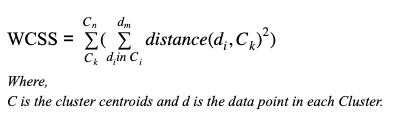
\includegraphics{"./U5A1-K-means_clustering_files/wcss.png"}
\caption{image.png}
\end{figure}

Once the \emph{no. of clusters vs WCSS} relationship is plotted, value
of \emph{K} can be found by looking the ``elbow''. ie; the point where
the discrete difference becomes gradual.

    \begin{tcolorbox}[breakable, size=fbox, boxrule=1pt, pad at break*=1mm,colback=cellbackground, colframe=cellborder]
\prompt{In}{incolor}{46}{\boxspacing}
\begin{Verbatim}[commandchars=\\\{\}]
\PY{n}{wcss} \PY{o}{=} \PY{p}{[}\PY{p}{]}
\PY{k}{for} \PY{n}{i} \PY{o+ow}{in} \PY{n+nb}{range}\PY{p}{(}\PY{l+m+mi}{1}\PY{p}{,}\PY{l+m+mi}{11}\PY{p}{)}\PY{p}{:}
    \PY{n}{kmeans} \PY{o}{=} \PY{n}{KMeans}\PY{p}{(}\PY{n}{n\PYZus{}clusters}\PY{o}{=}\PY{n}{i}\PY{p}{,} 
                    \PY{n}{init}\PY{o}{=}\PY{l+s+s1}{\PYZsq{}}\PY{l+s+s1}{k\PYZhy{}means++}\PY{l+s+s1}{\PYZsq{}}\PY{p}{,} \PY{c+c1}{\PYZsh{}init=\PYZsq{}random\PYZsq{},}
                    \PY{n}{max\PYZus{}iter}\PY{o}{=}\PY{l+m+mi}{300}\PY{p}{,} 
                    \PY{n}{n\PYZus{}init}\PY{o}{=}\PY{l+m+mi}{12}\PY{p}{,} 
                    \PY{n}{random\PYZus{}state}\PY{o}{=}\PY{l+m+mi}{0}\PY{p}{)}
    \PY{n}{kmeans}\PY{o}{.}\PY{n}{fit}\PY{p}{(}\PY{n}{X\PYZus{}ss}\PY{p}{)}
    \PY{n}{wcss}\PY{o}{.}\PY{n}{append}\PY{p}{(}\PY{n}{kmeans}\PY{o}{.}\PY{n}{inertia\PYZus{}}\PY{p}{)}
\PY{n}{f3}\PY{p}{,} \PY{n}{ax} \PY{o}{=} \PY{n}{plt}\PY{o}{.}\PY{n}{subplots}\PY{p}{(}\PY{n}{figsize}\PY{o}{=}\PY{p}{(}\PY{l+m+mi}{12}\PY{p}{,} \PY{l+m+mi}{6}\PY{p}{)}\PY{p}{)}
\PY{n}{plt}\PY{o}{.}\PY{n}{plot}\PY{p}{(}\PY{n+nb}{range}\PY{p}{(}\PY{l+m+mi}{1}\PY{p}{,}\PY{l+m+mi}{11}\PY{p}{)}\PY{p}{,}\PY{n}{wcss}\PY{p}{)}
\PY{c+c1}{\PYZsh{}plt.plot(range(1,10),diff(wcss))}
\PY{n}{plt}\PY{o}{.}\PY{n}{scatter}\PY{p}{(}\PY{l+m+mi}{3}\PY{p}{,} \PY{n}{wcss}\PY{p}{[}\PY{l+m+mi}{2}\PY{p}{]}\PY{p}{,} \PY{n}{marker}\PY{o}{=}\PY{l+s+s1}{\PYZsq{}}\PY{l+s+s1}{X}\PY{l+s+s1}{\PYZsq{}}\PY{p}{,} \PY{n}{c}\PY{o}{=}\PY{l+s+s1}{\PYZsq{}}\PY{l+s+s1}{r}\PY{l+s+s1}{\PYZsq{}}\PY{p}{)} 
\PY{n}{plt}\PY{o}{.}\PY{n}{title}\PY{p}{(}\PY{l+s+s1}{\PYZsq{}}\PY{l+s+s1}{The Elbow Method}\PY{l+s+s1}{\PYZsq{}}\PY{p}{)}
\PY{n}{plt}\PY{o}{.}\PY{n}{xlabel}\PY{p}{(}\PY{l+s+s1}{\PYZsq{}}\PY{l+s+s1}{Number of clusters}\PY{l+s+s1}{\PYZsq{}}\PY{p}{)}
\PY{n}{plt}\PY{o}{.}\PY{n}{ylabel}\PY{p}{(}\PY{l+s+s1}{\PYZsq{}}\PY{l+s+s1}{WCSS}\PY{l+s+s1}{\PYZsq{}}\PY{p}{)}
\PY{n}{plt}\PY{o}{.}\PY{n}{show}\PY{p}{(}\PY{p}{)}
\end{Verbatim}
\end{tcolorbox}

    \begin{center}
    \adjustimage{max size={0.9\linewidth}{0.9\paperheight}}{U5A1-K-means_clustering_files/U5A1-K-means_clustering_14_0.png}
    \end{center}
    { \hspace*{\fill} \\}
    
    In the above plot it can be noted that optimal number of clusters is 3.

    \hypertarget{c.-using-the-optimum-number-of-clusters-try-to-use-k-means-to-cluster-the-dataset-and-plot-a-2d-and-3d-plots-of-the-clusters-below.}{%
\subsubsection{c.~Using the optimum number of clusters, try to use
k-means to cluster the dataset and plot a 2D and 3D plots of the
clusters
below.}\label{c.-using-the-optimum-number-of-clusters-try-to-use-k-means-to-cluster-the-dataset-and-plot-a-2d-and-3d-plots-of-the-clusters-below.}}

\hypertarget{building-model-with-n_cluster3}{%
\paragraph{\texorpdfstring{Building model with
\texttt{n\_cluster=3}}{Building model with n\_cluster=3}}\label{building-model-with-n_cluster3}}

    \begin{tcolorbox}[breakable, size=fbox, boxrule=1pt, pad at break*=1mm,colback=cellbackground, colframe=cellborder]
\prompt{In}{incolor}{47}{\boxspacing}
\begin{Verbatim}[commandchars=\\\{\}]
\PY{n}{k\PYZus{}means} \PY{o}{=} \PY{n}{KMeans}\PY{p}{(}\PY{n}{init}\PY{o}{=}\PY{l+s+s1}{\PYZsq{}}\PY{l+s+s1}{k\PYZhy{}means++}\PY{l+s+s1}{\PYZsq{}}\PY{p}{,} \PY{n}{n\PYZus{}clusters}\PY{o}{=}\PY{l+m+mi}{3}\PY{p}{,} \PY{n}{n\PYZus{}init}\PY{o}{=}\PY{l+m+mi}{12}\PY{p}{,} \PY{n}{random\PYZus{}state}\PY{o}{=}\PY{l+m+mi}{0}\PY{p}{,} \PY{n}{max\PYZus{}iter}\PY{o}{=}\PY{l+m+mi}{1000}\PY{p}{)}
\PY{n}{k\PYZus{}means}\PY{o}{.}\PY{n}{fit}\PY{p}{(}\PY{n}{X\PYZus{}ss}\PY{p}{)}
\PY{n}{labels} \PY{o}{=} \PY{n}{k\PYZus{}means}\PY{o}{.}\PY{n}{labels\PYZus{}}

\PY{n}{df}\PY{p}{[}\PY{l+s+s1}{\PYZsq{}}\PY{l+s+s1}{pred\PYZus{}cluster}\PY{l+s+s1}{\PYZsq{}}\PY{p}{]} \PY{o}{=} \PY{n}{pd}\PY{o}{.}\PY{n}{Series}\PY{p}{(}\PY{n}{labels}\PY{p}{,} \PY{n}{index}\PY{o}{=}\PY{n}{df}\PY{o}{.}\PY{n}{index}\PY{p}{)} \PY{c+c1}{\PYZsh{}labels}
\PY{n}{df}\PY{p}{[}\PY{l+s+s1}{\PYZsq{}}\PY{l+s+s1}{pred\PYZus{}cluster}\PY{l+s+s1}{\PYZsq{}}\PY{p}{]} \PY{o}{=} \PY{n}{df}\PY{p}{[}\PY{l+s+s1}{\PYZsq{}}\PY{l+s+s1}{pred\PYZus{}cluster}\PY{l+s+s1}{\PYZsq{}}\PY{p}{]}\PY{o}{.}\PY{n}{map}\PY{p}{(}\PY{p}{\PYZob{}}\PY{l+m+mi}{0}\PY{p}{:} \PY{l+m+mi}{1}\PY{p}{,} \PY{l+m+mi}{1}\PY{p}{:} \PY{l+m+mi}{2}\PY{p}{,} \PY{l+m+mi}{2}\PY{p}{:} \PY{l+m+mi}{3}\PY{p}{\PYZcb{}}\PY{p}{)} \PY{c+c1}{\PYZsh{}mapping to keep cultivar names similar across predicted and ground truth }

\PY{n+nb}{print}\PY{p}{(}\PY{l+s+s2}{\PYZdq{}}\PY{l+s+s2}{Predicted Clusters}\PY{l+s+s2}{\PYZdq{}}\PY{p}{)}
\PY{n+nb}{print}\PY{p}{(}\PY{l+s+s2}{\PYZdq{}}\PY{l+s+s2}{=}\PY{l+s+s2}{\PYZdq{}}\PY{o}{*}\PY{l+m+mi}{74}\PY{p}{)}
\PY{n+nb}{print}\PY{p}{(}\PY{n}{df}\PY{p}{[}\PY{l+s+s2}{\PYZdq{}}\PY{l+s+s2}{pred\PYZus{}cluster}\PY{l+s+s2}{\PYZdq{}}\PY{p}{]}\PY{o}{.}\PY{n}{values}\PY{p}{)}
\PY{n+nb}{print}\PY{p}{(}\PY{l+s+s2}{\PYZdq{}}\PY{l+s+s2}{True Clusters}\PY{l+s+s2}{\PYZdq{}}\PY{p}{)}
\PY{n+nb}{print}\PY{p}{(}\PY{l+s+s2}{\PYZdq{}}\PY{l+s+s2}{=}\PY{l+s+s2}{\PYZdq{}}\PY{o}{*}\PY{l+m+mi}{74}\PY{p}{)}
\PY{n+nb}{print}\PY{p}{(}\PY{n}{df}\PY{p}{[}\PY{l+s+s1}{\PYZsq{}}\PY{l+s+s1}{Cultivar}\PY{l+s+s1}{\PYZsq{}}\PY{p}{]}\PY{o}{.}\PY{n}{values}\PY{p}{)}
\end{Verbatim}
\end{tcolorbox}

    \begin{Verbatim}[commandchars=\\\{\}]
Predicted Clusters
==========================================================================
[1 1 1 1 1 1 1 1 1 1 1 1 1 1 1 1 1 1 1 1 1 1 1 1 1 1 1 1 1 1 1 1 1 1 1 1 1
 1 1 1 1 1 1 1 1 1 1 1 1 1 1 1 1 1 1 1 1 1 1 2 2 3 2 2 2 2 2 2 2 2 2 2 2 1
 2 2 2 2 2 2 2 2 2 3 2 2 2 2 2 2 2 2 2 2 2 1 2 2 2 2 2 2 2 2 2 2 2 2 2 2 2
 2 2 2 2 2 2 2 3 2 2 1 2 2 2 2 2 2 2 2 3 3 3 3 3 3 3 3 3 3 3 3 3 3 3 3 3 3
 3 3 3 3 3 3 3 3 3 3 3 3 3 3 3 3 3 3 3 3 3 3 3 3 3 3 3 3 3 3]
True Clusters
==========================================================================
[1 1 1 1 1 1 1 1 1 1 1 1 1 1 1 1 1 1 1 1 1 1 1 1 1 1 1 1 1 1 1 1 1 1 1 1 1
 1 1 1 1 1 1 1 1 1 1 1 1 1 1 1 1 1 1 1 1 1 1 2 2 2 2 2 2 2 2 2 2 2 2 2 2 2
 2 2 2 2 2 2 2 2 2 2 2 2 2 2 2 2 2 2 2 2 2 2 2 2 2 2 2 2 2 2 2 2 2 2 2 2 2
 2 2 2 2 2 2 2 2 2 2 2 2 2 2 2 2 2 2 2 3 3 3 3 3 3 3 3 3 3 3 3 3 3 3 3 3 3
 3 3 3 3 3 3 3 3 3 3 3 3 3 3 3 3 3 3 3 3 3 3 3 3 3 3 3 3 3 3]
    \end{Verbatim}

    \hypertarget{d-plot}{%
\paragraph{2D Plot}\label{d-plot}}

    \begin{tcolorbox}[breakable, size=fbox, boxrule=1pt, pad at break*=1mm,colback=cellbackground, colframe=cellborder]
\prompt{In}{incolor}{48}{\boxspacing}
\begin{Verbatim}[commandchars=\\\{\}]
\PY{k}{def} \PY{n+nf}{cluster2D}\PY{p}{(}\PY{n}{x\PYZus{}label}\PY{p}{,} \PY{n}{y\PYZus{}label}\PY{p}{)}\PY{p}{:}
    \PY{n}{fig}\PY{p}{,} \PY{p}{(}\PY{n}{ax1}\PY{p}{,} \PY{n}{ax2}\PY{p}{)} \PY{o}{=} \PY{n}{plt}\PY{o}{.}\PY{n}{subplots}\PY{p}{(}\PY{l+m+mi}{1}\PY{p}{,} \PY{l+m+mi}{2}\PY{p}{,} \PY{n}{sharey}\PY{o}{=}\PY{k+kc}{True}\PY{p}{,} \PY{n}{figsize}\PY{o}{=}\PY{p}{(}\PY{l+m+mi}{12}\PY{p}{,} \PY{l+m+mi}{5}\PY{p}{)}\PY{p}{)}
    \PY{n}{sns}\PY{o}{.}\PY{n}{scatterplot}\PY{p}{(}\PY{n}{x}\PY{o}{=}\PY{n}{x\PYZus{}label}\PY{p}{,} \PY{n}{y}\PY{o}{=}\PY{n}{y\PYZus{}label}\PY{p}{,} \PY{n}{data}\PY{o}{=}\PY{n}{df}\PY{p}{,} \PY{n}{hue}\PY{o}{=}\PY{l+s+s1}{\PYZsq{}}\PY{l+s+s1}{pred\PYZus{}cluster}\PY{l+s+s1}{\PYZsq{}}\PY{p}{,} \PY{n}{palette}\PY{o}{=}\PY{l+s+s2}{\PYZdq{}}\PY{l+s+s2}{Set2}\PY{l+s+s2}{\PYZdq{}}\PY{p}{,} \PY{n}{ax}\PY{o}{=}\PY{n}{ax1}\PY{p}{)}
    \PY{n}{wrong\PYZus{}cluster} \PY{o}{=} \PY{n}{df}\PY{p}{[}\PY{n}{df}\PY{p}{[}\PY{l+s+s1}{\PYZsq{}}\PY{l+s+s1}{pred\PYZus{}cluster}\PY{l+s+s1}{\PYZsq{}}\PY{p}{]} \PY{o}{!=} \PY{n}{df}\PY{p}{[}\PY{l+s+s1}{\PYZsq{}}\PY{l+s+s1}{Cultivar}\PY{l+s+s1}{\PYZsq{}}\PY{p}{]}\PY{p}{]}
    \PY{n}{sns}\PY{o}{.}\PY{n}{scatterplot}\PY{p}{(}\PY{n}{x}\PY{o}{=}\PY{n}{x\PYZus{}label}\PY{p}{,} \PY{n}{y}\PY{o}{=}\PY{n}{y\PYZus{}label}\PY{p}{,} \PY{n}{data}\PY{o}{=}\PY{n}{df}\PY{p}{,} \PY{n}{hue}\PY{o}{=}\PY{l+s+s1}{\PYZsq{}}\PY{l+s+s1}{Cultivar}\PY{l+s+s1}{\PYZsq{}}\PY{p}{,} \PY{n}{palette}\PY{o}{=}\PY{l+s+s2}{\PYZdq{}}\PY{l+s+s2}{Set2}\PY{l+s+s2}{\PYZdq{}}\PY{p}{,} \PY{n}{ax}\PY{o}{=}\PY{n}{ax2}\PY{p}{)}
    \PY{n}{ax1}\PY{o}{.}\PY{n}{title}\PY{o}{.}\PY{n}{set\PYZus{}text}\PY{p}{(}\PY{l+s+s1}{\PYZsq{}}\PY{l+s+s1}{Predicted Cluster}\PY{l+s+s1}{\PYZsq{}}\PY{p}{)}
    \PY{n}{ax2}\PY{o}{.}\PY{n}{title}\PY{o}{.}\PY{n}{set\PYZus{}text}\PY{p}{(}\PY{l+s+s1}{\PYZsq{}}\PY{l+s+s1}{True Cluster}\PY{l+s+s1}{\PYZsq{}}\PY{p}{)}
    \PY{n}{ax1}\PY{o}{.}\PY{n}{scatter}\PY{p}{(}\PY{n}{wrong\PYZus{}cluster}\PY{p}{[}\PY{n}{x\PYZus{}label}\PY{p}{]}\PY{p}{,} \PY{n}{wrong\PYZus{}cluster}\PY{p}{[}\PY{n}{y\PYZus{}label}\PY{p}{]}\PY{p}{,} \PY{n}{s}\PY{o}{=}\PY{l+m+mi}{80}\PY{p}{,} \PY{n}{facecolors}\PY{o}{=}\PY{l+s+s1}{\PYZsq{}}\PY{l+s+s1}{none}\PY{l+s+s1}{\PYZsq{}}\PY{p}{,} \PY{n}{edgecolors}\PY{o}{=}\PY{l+s+s1}{\PYZsq{}}\PY{l+s+s1}{r}\PY{l+s+s1}{\PYZsq{}}\PY{p}{)}
    \PY{n}{ax2}\PY{o}{.}\PY{n}{scatter}\PY{p}{(}\PY{n}{wrong\PYZus{}cluster}\PY{p}{[}\PY{n}{x\PYZus{}label}\PY{p}{]}\PY{p}{,} \PY{n}{wrong\PYZus{}cluster}\PY{p}{[}\PY{n}{y\PYZus{}label}\PY{p}{]}\PY{p}{,} \PY{n}{s}\PY{o}{=}\PY{l+m+mi}{80}\PY{p}{,} \PY{n}{facecolors}\PY{o}{=}\PY{l+s+s1}{\PYZsq{}}\PY{l+s+s1}{none}\PY{l+s+s1}{\PYZsq{}}\PY{p}{,} \PY{n}{edgecolors}\PY{o}{=}\PY{l+s+s1}{\PYZsq{}}\PY{l+s+s1}{r}\PY{l+s+s1}{\PYZsq{}}\PY{p}{)}
    \PY{c+c1}{\PYZsh{}ax1.scatter(k\PYZus{}means.cluster\PYZus{}centers\PYZus{}[:, 0], k\PYZus{}means.cluster\PYZus{}centers\PYZus{}[:, 1],}
    \PY{c+c1}{\PYZsh{}            s=100, c=\PYZsq{}cyan\PYZsq{}, label = \PYZsq{}Centroids\PYZsq{})}
    \PY{k}{for} \PY{n}{i}\PY{p}{,} \PY{n}{row} \PY{o+ow}{in} \PY{n}{wrong\PYZus{}cluster}\PY{o}{.}\PY{n}{iterrows}\PY{p}{(}\PY{p}{)}\PY{p}{:}
        \PY{n}{xy} \PY{o}{=} \PY{p}{(}\PY{n}{row}\PY{p}{[}\PY{n}{x\PYZus{}label}\PY{p}{]}\PY{p}{,} \PY{n}{row}\PY{p}{[}\PY{n}{y\PYZus{}label}\PY{p}{]}\PY{p}{)}
        \PY{n}{con} \PY{o}{=} \PY{n}{ConnectionPatch}\PY{p}{(}\PY{n}{xyA}\PY{o}{=}\PY{n}{xy}\PY{p}{,} \PY{n}{xyB}\PY{o}{=}\PY{n}{xy}\PY{p}{,} \PY{n}{coordsA}\PY{o}{=}\PY{l+s+s2}{\PYZdq{}}\PY{l+s+s2}{data}\PY{l+s+s2}{\PYZdq{}}\PY{p}{,} \PY{n}{coordsB}\PY{o}{=}\PY{l+s+s2}{\PYZdq{}}\PY{l+s+s2}{data}\PY{l+s+s2}{\PYZdq{}}\PY{p}{,}
                              \PY{n}{axesA}\PY{o}{=}\PY{n}{ax2}\PY{p}{,} \PY{n}{axesB}\PY{o}{=}\PY{n}{ax1}\PY{p}{,} \PY{n}{color}\PY{o}{=}\PY{l+s+s2}{\PYZdq{}}\PY{l+s+s2}{red}\PY{l+s+s2}{\PYZdq{}}\PY{p}{)}
        \PY{n}{ax2}\PY{o}{.}\PY{n}{add\PYZus{}artist}\PY{p}{(}\PY{n}{con}\PY{p}{)}
    \PY{n}{super\PYZus{}title} \PY{o}{=} \PY{n}{x\PYZus{}label} \PY{o}{+} \PY{l+s+s2}{\PYZdq{}}\PY{l+s+s2}{ vs }\PY{l+s+s2}{\PYZdq{}} \PY{o}{+} \PY{n}{y\PYZus{}label}
    \PY{n}{super\PYZus{}title} \PY{o}{+}\PY{o}{=} \PY{n}{f}\PY{l+s+s2}{\PYZdq{}}\PY{l+s+se}{\PYZbs{}n}\PY{l+s+s2}{Wrongly clustered = }\PY{l+s+s2}{\PYZob{}}\PY{l+s+s2}{len(wrong\PYZus{}cluster)\PYZcb{}/}\PY{l+s+s2}{\PYZob{}}\PY{l+s+s2}{len(df)\PYZcb{}}\PY{l+s+s2}{\PYZdq{}}
    \PY{n}{fig}\PY{o}{.}\PY{n}{suptitle}\PY{p}{(}\PY{n}{super\PYZus{}title}\PY{p}{)}
        
    

\PY{n}{cluster2D}\PY{p}{(}\PY{l+s+s1}{\PYZsq{}}\PY{l+s+s1}{Alcohol}\PY{l+s+s1}{\PYZsq{}}\PY{p}{,} \PY{l+s+s1}{\PYZsq{}}\PY{l+s+s1}{OD280/OD315}\PY{l+s+s1}{\PYZsq{}}\PY{p}{)}
\PY{n}{cluster2D}\PY{p}{(}\PY{l+s+s1}{\PYZsq{}}\PY{l+s+s1}{Alcohol}\PY{l+s+s1}{\PYZsq{}}\PY{p}{,} \PY{l+s+s1}{\PYZsq{}}\PY{l+s+s1}{Flavanoids}\PY{l+s+s1}{\PYZsq{}}\PY{p}{)}
\PY{n}{cluster2D}\PY{p}{(}\PY{l+s+s1}{\PYZsq{}}\PY{l+s+s1}{Alcohol}\PY{l+s+s1}{\PYZsq{}}\PY{p}{,} \PY{l+s+s1}{\PYZsq{}}\PY{l+s+s1}{Proline}\PY{l+s+s1}{\PYZsq{}}\PY{p}{)}
\end{Verbatim}
\end{tcolorbox}

    \begin{center}
    \adjustimage{max size={0.9\linewidth}{0.9\paperheight}}{U5A1-K-means_clustering_files/U5A1-K-means_clustering_19_0.png}
    \end{center}
    { \hspace*{\fill} \\}
    
    \begin{center}
    \adjustimage{max size={0.9\linewidth}{0.9\paperheight}}{U5A1-K-means_clustering_files/U5A1-K-means_clustering_19_1.png}
    \end{center}
    { \hspace*{\fill} \\}
    
    \begin{center}
    \adjustimage{max size={0.9\linewidth}{0.9\paperheight}}{U5A1-K-means_clustering_files/U5A1-K-means_clustering_19_2.png}
    \end{center}
    { \hspace*{\fill} \\}
    
    \textbf{Observation}

From the plots it can be observed that all the wrong clustering happened
to \texttt{Cultivar\ \#2}.

    \hypertarget{d-plot}{%
\paragraph{3D Plot}\label{d-plot}}

\hypertarget{plot-alcohol-od280od315-proline}{%
\subparagraph{\texorpdfstring{Plot
\texttt{\textquotesingle{}Alcohol\textquotesingle{},\ \textquotesingle{}OD280/OD315\textquotesingle{},\ \textquotesingle{}Proline\textquotesingle{}}}{Plot 'Alcohol', 'OD280/OD315', 'Proline'}}\label{plot-alcohol-od280od315-proline}}

    \begin{tcolorbox}[breakable, size=fbox, boxrule=1pt, pad at break*=1mm,colback=cellbackground, colframe=cellborder]
\prompt{In}{incolor}{58}{\boxspacing}
\begin{Verbatim}[commandchars=\\\{\}]
\PY{k}{def} \PY{n+nf}{cluster3D}\PY{p}{(}\PY{n}{x\PYZus{}label}\PY{p}{,} \PY{n}{y\PYZus{}label}\PY{p}{,} \PY{n}{z\PYZus{}label}\PY{p}{)}\PY{p}{:}
    \PY{n}{f4} \PY{o}{=} \PY{n}{plt}\PY{o}{.}\PY{n}{figure}\PY{p}{(}\PY{l+m+mi}{1}\PY{p}{,} \PY{n}{figsize}\PY{o}{=}\PY{p}{(}\PY{l+m+mi}{10}\PY{p}{,} \PY{l+m+mi}{8}\PY{p}{)}\PY{p}{)}
    \PY{n}{plt}\PY{o}{.}\PY{n}{clf}\PY{p}{(}\PY{p}{)}
    \PY{n}{ax} \PY{o}{=} \PY{n}{Axes3D}\PY{p}{(}\PY{n}{f4}\PY{p}{,} \PY{n}{rect}\PY{o}{=}\PY{p}{[}\PY{l+m+mi}{0}\PY{p}{,} \PY{l+m+mi}{0}\PY{p}{,} \PY{o}{.}\PY{l+m+mi}{95}\PY{p}{,} \PY{l+m+mi}{1}\PY{p}{]}\PY{p}{,} \PY{n}{elev}\PY{o}{=}\PY{l+m+mi}{48}\PY{p}{,} \PY{n}{azim}\PY{o}{=}\PY{l+m+mi}{134}\PY{p}{)}

    \PY{n}{plt}\PY{o}{.}\PY{n}{cla}\PY{p}{(}\PY{p}{)}
    \PY{n}{ax}\PY{o}{.}\PY{n}{set\PYZus{}xlabel}\PY{p}{(}\PY{n}{x\PYZus{}label}\PY{p}{)}
    \PY{n}{ax}\PY{o}{.}\PY{n}{set\PYZus{}ylabel}\PY{p}{(}\PY{n}{y\PYZus{}label}\PY{p}{)}
    \PY{n}{ax}\PY{o}{.}\PY{n}{set\PYZus{}zlabel}\PY{p}{(}\PY{n}{z\PYZus{}label}\PY{p}{)}

    \PY{n}{ax}\PY{o}{.}\PY{n}{scatter}\PY{p}{(}\PY{n}{df}\PY{p}{[}\PY{n}{x\PYZus{}label}\PY{p}{]}\PY{p}{,} \PY{n}{df}\PY{p}{[}\PY{n}{y\PYZus{}label}\PY{p}{]}\PY{p}{,} \PY{n}{df}\PY{p}{[}\PY{n}{z\PYZus{}label}\PY{p}{]}\PY{p}{,} \PY{n}{c}\PY{o}{=}\PY{n}{df}\PY{p}{[}\PY{l+s+s1}{\PYZsq{}}\PY{l+s+s1}{pred\PYZus{}cluster}\PY{l+s+s1}{\PYZsq{}}\PY{p}{]}\PY{p}{,} \PY{n}{s}\PY{o}{=}\PY{l+m+mi}{80}\PY{p}{)}

\PY{n}{cluster3D}\PY{p}{(}\PY{l+s+s1}{\PYZsq{}}\PY{l+s+s1}{Alcohol}\PY{l+s+s1}{\PYZsq{}}\PY{p}{,} \PY{l+s+s1}{\PYZsq{}}\PY{l+s+s1}{OD280/OD315}\PY{l+s+s1}{\PYZsq{}}\PY{p}{,} \PY{l+s+s1}{\PYZsq{}}\PY{l+s+s1}{Proline}\PY{l+s+s1}{\PYZsq{}}\PY{p}{)}
\end{Verbatim}
\end{tcolorbox}

    \begin{center}
    \adjustimage{max size={0.9\linewidth}{0.9\paperheight}}{U5A1-K-means_clustering_files/U5A1-K-means_clustering_22_0.png}
    \end{center}
    { \hspace*{\fill} \\}
    
    \hypertarget{plot-malic-acid-ash-alcalinity-of-ash}{%
\subparagraph{\texorpdfstring{Plot
\texttt{"Malic\ acid",\ "Ash",\ "Alcalinity\ of\ ash"}}{Plot "Malic acid", "Ash", "Alcalinity of ash"}}\label{plot-malic-acid-ash-alcalinity-of-ash}}

    \begin{tcolorbox}[breakable, size=fbox, boxrule=1pt, pad at break*=1mm,colback=cellbackground, colframe=cellborder]
\prompt{In}{incolor}{53}{\boxspacing}
\begin{Verbatim}[commandchars=\\\{\}]
\PY{n}{cluster3D}\PY{p}{(}\PY{l+s+s2}{\PYZdq{}}\PY{l+s+s2}{Malic acid}\PY{l+s+s2}{\PYZdq{}}\PY{p}{,} \PY{l+s+s2}{\PYZdq{}}\PY{l+s+s2}{Ash}\PY{l+s+s2}{\PYZdq{}}\PY{p}{,} \PY{l+s+s2}{\PYZdq{}}\PY{l+s+s2}{Alcalinity of ash}\PY{l+s+s2}{\PYZdq{}}\PY{p}{)}
\end{Verbatim}
\end{tcolorbox}

    \begin{center}
    \adjustimage{max size={0.9\linewidth}{0.9\paperheight}}{U5A1-K-means_clustering_files/U5A1-K-means_clustering_24_0.png}
    \end{center}
    { \hspace*{\fill} \\}
    
    \hypertarget{plot-color-intensity-hue-od280od315}{%
\subparagraph{\texorpdfstring{Plot
\texttt{"Color\ intensity",\ "Hue",\ "OD280/OD315"}}{Plot "Color intensity", "Hue", "OD280/OD315"}}\label{plot-color-intensity-hue-od280od315}}

    \begin{tcolorbox}[breakable, size=fbox, boxrule=1pt, pad at break*=1mm,colback=cellbackground, colframe=cellborder]
\prompt{In}{incolor}{55}{\boxspacing}
\begin{Verbatim}[commandchars=\\\{\}]
\PY{n}{cluster3D}\PY{p}{(}\PY{l+s+s2}{\PYZdq{}}\PY{l+s+s2}{Color intensity}\PY{l+s+s2}{\PYZdq{}}\PY{p}{,} \PY{l+s+s2}{\PYZdq{}}\PY{l+s+s2}{Hue}\PY{l+s+s2}{\PYZdq{}}\PY{p}{,} \PY{l+s+s2}{\PYZdq{}}\PY{l+s+s2}{OD280/OD315}\PY{l+s+s2}{\PYZdq{}}\PY{p}{)}
\end{Verbatim}
\end{tcolorbox}

    \begin{center}
    \adjustimage{max size={0.9\linewidth}{0.9\paperheight}}{U5A1-K-means_clustering_files/U5A1-K-means_clustering_26_0.png}
    \end{center}
    { \hspace*{\fill} \\}
    
    The clustering was done in a 13-dimensional space. We try to represent a
few subsets of those 13 features in the 2D and 3D plots above. It can be
observed that while some of these plots have clear separation between
clusters (eg. \texttt{Alcohol}, \texttt{OD280/OD315}, \texttt{Proline})
others don't (eg. \texttt{Color\ intensity}, \texttt{Hue},
\texttt{OD280/OD315}).

From this it can be infered that the clustering algorithm might provide
similar results even with a fewer number of features.

    \hypertarget{marks-what-are-the-new-things-that-you-learned-by-doing-this-assignment.-list-down-at-least-3-bullet-points.}{%
\subsection{{[}2 MARKS{]} What are the new things that you learned by
doing this assignment. List down at least 3 bullet
points.}\label{marks-what-are-the-new-things-that-you-learned-by-doing-this-assignment.-list-down-at-least-3-bullet-points.}}

\begin{itemize}
\tightlist
\item
  To implement k-mean clustering with scikit learn Kmeans()
\item
  Selecting the correct value of K (the number of clusters) using the
  \emph{elbow method}
\item
  Intuition behind the \emph{elbow method}
\item
  Various methods to intialize centroids (\texttt{k-means++},
  \texttt{random} etc)
\end{itemize}


    % Add a bibliography block to the postdoc
    
    
    
\end{document}
